\documentclass{jsarticle}
\usepackage[top=20truemm,bottom=20truemm,left=25truemm,right=25truemm]{geometry}
\usepackage{amsmath,ascmac,url,amsfonts,bm,here,algorithmic,algorithm,amsthm,color}
\usepackage[dvipdfmx]{graphicx}
\newcommand{\argmax}{\mathop{\rm argmax}\limits}
\newcommand{\argmin}{\mathop{\rm argmin}\limits} 
\newcommand{\expect}{\mathbb{E}} 
\newcommand{\trans}[1]{#1^{\top}}
\newcommand{\pdif}[2]{\frac{\partial#1}{\partial#2}}
\newcommand{\odif}[2]{\frac{\rm{d}#1}{\rm{d}#2}}
\makeatletter
  \def\@maketitle{
  \newpage\null
  \vskip 2em
    \mbox{}\hfill
    \begin{flushleft}
    \textbf{制御システム論分野研究会資料}
    \end{flushleft}
    \begin{flushright}
    {\lineskip .5em
      \begin{tabular}[t]{c}
        \@date \\
        \@author
      \end{tabular}\par}
        \end{flushright}
  \begin{center}
  \let\footnote\thanks
    {\LARGE \@title \par}
    \vskip 1.5em
  \end{center}
    \vskip 1em
  \par}
\makeatother
\title{\large{\bf{進捗報告 8.20}}}
\author{M2 竹内 維吹}
%\date{Jul. 7, 2020}
\date{\today}
\begin{document}
\maketitle


\section{問題設定(作成中)}
以下のような入力アフィン系システムを考える.
\begin{equation}
	\dot{s}=f(s)+g(s)a \label{true_dynamics}
\end{equation}
ここで,~$s_t, a_t$はそれぞれ状態ベクトル, 入力ベクトルである.\par
さらに, 図1のようなシステム(\ref{true_dynamics})に対するイベント駆動型制御を考える.
\begin{figure}[h]
	\centering
 	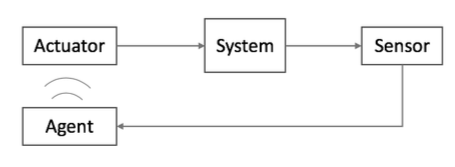
\includegraphics[width=8cm]{event.png}
 	\caption{イベント駆動型制御}
\end{figure}\\
ここではエージェントの制御則$\pi(s)$を設計するとし, $\pi(s)$はシステムに加えるべき入力信号$a$と, それを送信するかどうかを決定する2値変数$c~(c = 1 ならば送信)$で構成されるとする.つまり
\begin{equation}
	\pi(\cdot) = [~a, c~]^{\top}
\end{equation}
であるとする. このようなイベント駆動型制御に対して, 以下の条件を満たす最適イベント駆動型制御則$\pi^{*}(\cdot)$を導出する問題を考える.
\begin{align}
	\pi^{*}(\cdot) &= \argmax_{\pi}\expect_{s_0 \sim d_0}\left[V^{\pi} (s_0)\right] \label{optimal_policy}\\
	V^{\pi} (s_0) &=\sum_{t=0}^{\infty}(-s_t^{\top}Qs_t - \pi^{\top}(s_t)R\pi(s_t) - \lambda\gamma_t) \label{V}
\end{align}
ここで,~$\gamma_t$は時刻$t$においてエージェントがアクチュエータと通信を行ったかを表す2値変数である.また, $Q,R,\gamma$はそれぞれ正定値, 半正定値, 正のハイパーパラメータであり, $d_0$は初期状態を与える確率分布である.式(\ref{V})より, 「最小限の入力エネルギーで」かつ「最小限の通信回数で」「状態$s$を0に素早く漸近させる」と$V$が最大化される.\par
さて, システム(\ref{true_dynamics})が未知であるという設定のもとで, 実環境とのインタラクションによってデータ組$(s_t, a_t, r_t, s_{t+1})$を収集し, それらを活用することで上記の問題を解いていたのは\cite{event}である.\par
本研究ではさらに一歩踏み込んで, データ収集の実環境とのインタラクションの際に状態制約
\begin{equation}
	s\in C, C\subset S \label{constraint}
\end{equation}
を全時刻において満たしながら$\pi^{*}(\cdot)$を求める問題を考える.ただし, 式(\ref{optimal_policy})における$d_0$は$\textrm{support}(d_0)\subset C$を満たすとする.また, $S$は実環境において考えられうる全状態の集合であるとする.\par
\color{red}(現状, 上記の問題を解くことが研究の目標であると考えています.ただ, この先どのような仮定を置くかはまだ考えられていません. )

\color{black}
\section{DDPGとCBFを用いた解法}
システム(\ref{true_dynamics})に対して, 関数$h(s)$が以下の式を満たすならば,~$h(s)$は制御バリア関数(CBF)と呼ばれる.
\begin{equation}
	\sup_{a\in A}\left\{\pdif{h}{s}(f(s)+g(s)a)+K(h(s))\right\} \geq 0 \label{CBF}
\end{equation}
ただし, $K(s)$はクラスK関数である.\par
さて, 式(\ref{constraint})における状態制約$C$が
\begin{equation}
	C = \left\{s \in S~|~h(s)\geq 0\right\}
\end{equation}
として与えられているとする. このとき$h(s)$が制御バリア関数であるならば, 状態$s\in C$に対して次の時刻における状態$s^{\prime}$が$s^{\prime}\in C$を満たすようにする入力が存在することを保証する. そのような入力集合は現時刻での状態$s$に依存し,
\begin{equation}
	U(s) = \left\{a \in A~|~\pdif{h}{s}(f(s)+g(s)a)+K(h(s))\geq 0\right\}, \forall s\in C
\end{equation}
としてその集合を与える.\par
さて, DDPGなどの方策on型の強化学習では, 制御則$\pi(\cdot)$を用いて実環境とインタラクションを行い, データを収集・利活用することで, より$V^{\pi}$を大きくできるような制御則$\pi^{\prime}(\cdot)$を模索する.その過程で制御入力$\pi(s)$が$\pi(s)\notin U(s)$となるならば, 次時刻において状態制約$C$を満たさない状態に遷移してしまう.それを避けるため, $\pi(s)\notin U(s)$となった各時刻では, $\pi(s)$ではなく,~$\pi(s)$に最も近い$U(s)$の元を用いてインタラクションを行う手法を考えてみる.

\section{倒立振子による実験}
倒立時の振子の角度を$\theta=0$とし, 加えられる入力が$A=[-10\textrm{N}\cdot\textrm{m},10\textrm{N}\cdot\textrm{m}]$と制限されるような倒立振子を考える.この倒立振子のダイナミクスは, 以下のように与えられる.
\begin{align}
	\theta_{t+1} &= \theta_t+\dot{\theta}_t\delta_t+\frac{3g}{2l}\sin{\theta_t}\delta_t^2+\frac{3}{ml^2}a\delta_t^2 \\
	\dot{\theta}_{t+1} &=  \dot{\theta}_t+\frac{3g}{2l}\sin{\theta_t}\delta_t+\frac{3}{ml^2}a\delta_t
\end{align}
これは式(\ref{true_dynamics})に対応する. 本実験ではこのダイナミクスが既知であるとして$U(s)$を構築し, 状態制約(\ref{constraint})を満たしながら$\pi^{*}$を求めることができるのかを検証する. ただし, $\delta_t$は離散化定数であり$\delta_t=0.005$とする.\par
ただし, これは離散化された状態方程式であるため, CBFによる状態制約の前進不変性をより厳密に議論するために対応する連続時間システムを書き下すと
\begin{equation}
	\odif{}{t}\begin{pmatrix}\theta \\ \dot{\theta}\end{pmatrix} = 
		\begin{pmatrix}\dot{\theta} \\ \frac{3g}{2l}\sin{\theta} + \frac{3}{ml^2}a \end{pmatrix} \label{continuous}
\end{equation}
となる. 与えられた関数$h(s)$が制御バリア関数か否かを調べるには, 式(\ref{continuous})と式(\ref{CBF})を用いる.\par
さて, ~$s=[~\theta, \dot{\theta}~]^{\top}$とすると$S = \{s~|~\theta\in[-\pi, \pi], \dot{\theta}\in\mathbb{R}\}$である.ここで, 状態制約集合$C\in S$を
\begin{equation}
	C=\{s\in S~|~h(s)\geq 0\}
\end{equation}とし,~$h(s)=(1-\theta^2-\alpha\dot{\theta}^2), \alpha>0$とおく. すると, 状態制約集合$C$は以下のように分布する. 
\begin{figure}[h]
	\centering
 	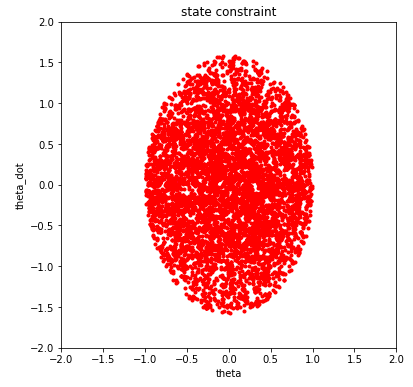
\includegraphics[width=6cm]{region.png}
 	\caption{状態集合$C$}
\end{figure}\\

式$(\ref{CBF})$における$K$を$K(x) = \gamma x$とおくと式(\ref{CBF})は次のようになる.
\begin{equation}
	\sup_{a\in A}\left\{-2\theta\dot{\theta}-\frac{3g\alpha}{l}\dot{\theta}\sin{\theta}-\frac{6\alpha}{ml^2}\dot{\theta} a+\gamma(1-\theta^2-\alpha\dot{\theta}^2)\right\} \geq 0 \label{special_cbf}
\end{equation}
括弧の中は$a$に関する1次式となっているため$\dot{\theta}$の正負に合わせて$U(s)$を定義できる($\frac{6\alpha}{ml^2}$は必ず正のため).\par
さて, 括弧の中身を
\begin{equation}
	p(a) = -2\theta\dot{\theta}-\frac{3g\alpha}{l}\dot{\theta}\sin{\theta}-\frac{6\alpha}{ml^2}\dot{\theta} a+\gamma(1-\theta^2-\alpha\dot{\theta}^2)
\end{equation}
としたとき, $p(a)=0$の解を$a^{*}$とすれば,~$a$は1次元なので$\theta<0$のとき$U(s)$は以下のようになる.
\begin{equation}
	U(s) = 
		\begin{cases}
			[~a^{*}, 10~]~~\textrm{if}~~ a^{*} > -10 \\
			[~-10, 10~]~~\textrm{if}~~ a^{*} \leq -10
		\end{cases}
\end{equation}
また, $\theta>0$のときも同様にすると
\begin{equation}
	U(s) = 
		\begin{cases}
			[~-10, a^{*}~]~~\textrm{if}~~ a^{*} < 10 \\
			[~-10, 10~]~~\textrm{if}~~ a^{*} \geq 10
		\end{cases}
\end{equation}
として与えることができる.

\section{実験結果}
Open-AI Gym Pendulum-v0とKeras-RLを用いてシミュレーションを行ったについて考察する. Keras-RLでは学習を行う合計ステップ数をいくつかのepisodeに分割する. ここではepisodeのステップを2000とし, 合計ステップを3000000に設定して実験を行った. 計算時間は1回あたり5,6時間である. 以下では(1):episodeを通して状態制約を満たしているのか, またその時CBFの働きはどうか. (2):イベント駆動制御がなされているか. (3):episodeを通しての蓄積rewardは増えているか.
という観点で結果を確認していく. 

\subsection{CBFによる入力射影ルールの変更}
ここまで状態$s$における制御入力$\pi(s)$が$U(s)$の元でない場合, $\pi(s)$ではなく, $U(s)$の元のうち最も$\pi(s)$近いものを, 実際にその時刻でシステムに加える入力だとしていた. しかしこの設定で学習を行っても, 方策の改善は見られなかった. 図\ref{pure_reward}は横軸をepisode, 縦軸を各episodeを通してのrewardとして, その変化を示したグラフである. オレンジ線は30episode移動平均線である. この図から, episodeを進めて行っても方策が改善せず, また振子を倒立させた(この時は0付近のepisode rewardになる)episodeがほとんどないことが見て取れる.
\begin{figure}[h]
	\centering
 	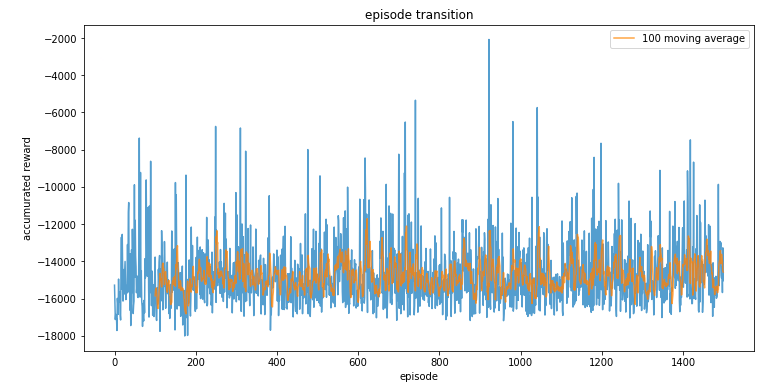
\includegraphics[width=12cm]{pure_reward.png}
 	\caption{episode毎の蓄積reward} \label{pure_reward}
\end{figure}\\

また, 3000000ステップの学習によって得られた$\pi(\cdot)$によって, 1episode内でどのような制御が行われるかを見てみる. 
\begin{figure}[h]
	\centering
 	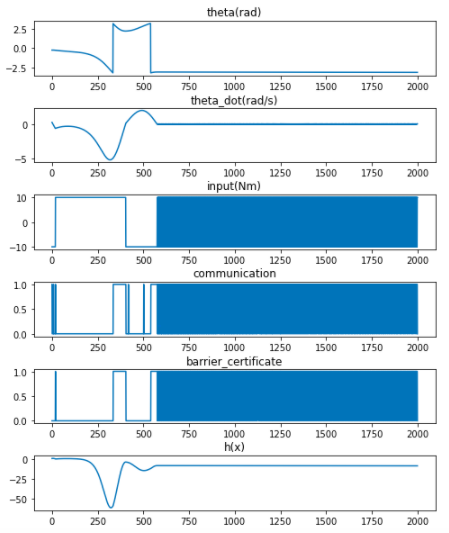
\includegraphics[width=10cm]{pure_control_log.png}
 	\caption{制御内容} \label{pure_control_log}
\end{figure}\\
図\ref{pure_control_log}は上段からそれぞれ$\theta, \dot{\theta}$, a(入力), 通信の有無, CBFによる入力射影の有無, 各時刻の$h(s)$が, 時間ステップ毎にどう変化するかを表したグラフである. 図から離散化の影響によって200ステップあたりから状態制約を満たさなくなってしまい, $\dot{\theta}$を0にすることによってrewardを大きくするという局所最適方策に陥っているように見える. \par

これを受けて, CBFによる入力射影ルールを少し改変した. これは$h(s)<0.1$となった時のみ, $U(s)$の元のうち最も$\pi(s)$近いものではなく, 最も効率の良い入力(例えば, $\theta<0$であれば$a=10$)を選ぶようにするというものである. 次節からはこの入力ルールによる学習の内容を示す.


\subsection{状態制約とCBF}
図\ref{init}にランダムに入力を返すような初期方策$\pi_0(\cdot)$によるepisodeの実績を示す. 両図ともに横軸はステップを示す. 上図はステップ毎に$h(s)$をプロットした図(参考に$y$座標が0となるラインをオレンジで引いている)である.下図はCBFによって$\pi_0(s_t)$が変更された場合に1, それ以外で0となるようにプロットした図である.
\begin{figure}[h]
	\centering
 	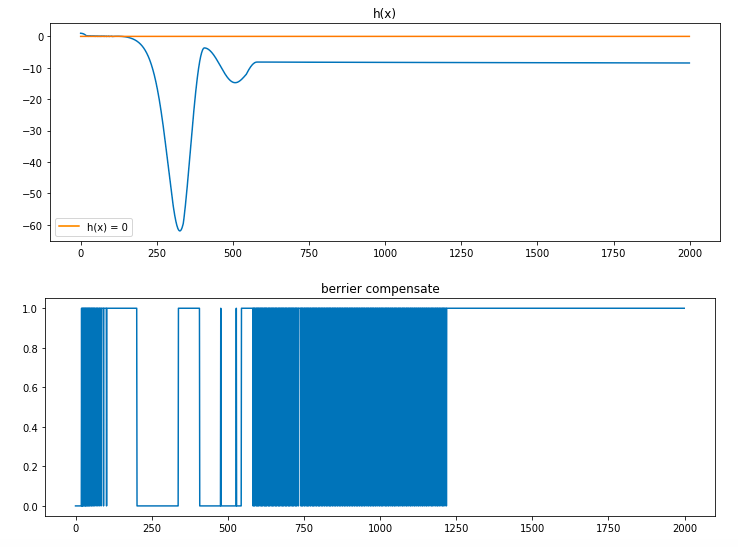
\includegraphics[width=10cm]{initial_policy.png}
 	\caption{学習初期の$\pi(\cdot)$の実績} \label{init}
\end{figure}\\

この図を見ると200ステップ目までは状態制約$h(s)\geq 0$を保てているが, それ以降では制約を満たせていない($h(s)<0$). 前節で述べたとおり, CBFは連続時間システムに対して成り立つ論理なので, 離散化したシミュレーションではその論理が破綻することがある.これはその影響である. \par

次に学習後期の方策方策$\pi_{t_{late}}(\cdot)$の実績を見てみる. 
\begin{figure}[h]
	\centering
 	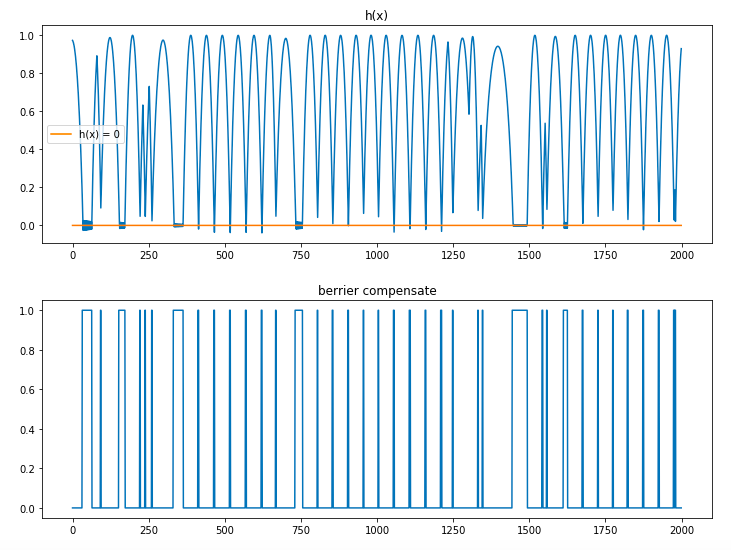
\includegraphics[width=10cm]{good_policy.png}
 	\caption{学習後期の$\pi(\cdot)$の実績}
\end{figure}\par
こちらではepisodeを通して状態制約$h(s)\geq 0$を保てている. 初期方策との違いは, ランダムな制御則ではなく, rewardを大きくしようとする制御則になっていることである. 状態制約が保たれる理由は, これにより制約集合内に留まろうとする回数が多くなり, 離散化によるCBFの破綻が起こる回数が少なくなっているためと考えられる.\par

最後に,全episodeを通して同じグラフを描いた結果を示す. \par
\begin{figure}[h]
	\centering
 	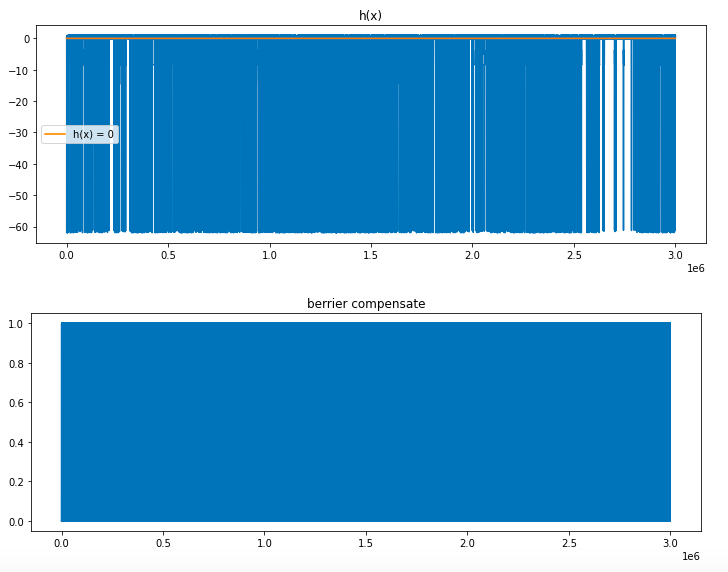
\includegraphics[width=10cm]{all_policies2.png}
 	\caption{全エピソードの実績}
\end{figure}\par

エピソードの始まりに,状態が$h(s_{init})>0$となるように選んでいるため, 各エピソードの開始時に強制的に$h$のグラフが0より大きくなる. 図5を見ると, 0以上から最小値付近に遷移する回数が, 後半になるにつれて少なくなっている.これは, 状態制約を保てる回数が増えていることを示し, エージェントが状態制約集合の中にある最適状態(倒立)を留めておける方策の学習を進めることができていることの表れだと考える. \par

\subsection{最適イベント駆動制御になっているか}
次に学習した方策はイベント駆動制御になっているのかを見てみる. \par
\begin{figure}[h]
	\centering
 	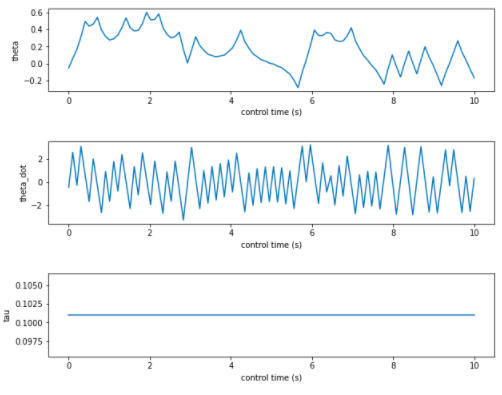
\includegraphics[width=10cm]{control_log.png}
 	\caption{制御内容} \label{control_log}
\end{figure}
図\ref{control_log}は図\ref{pure_control_log}と同じクラスのグラフである. 図\ref{control_log}の4段目を見ると通信を行っている回数が$10\%$ほどに抑えられており, イベント駆動制御になっていると言える. また, 1,2段目を見ると$\theta, \dot{\theta}$は0付近にとどまっており, 振り子が倒立していることを示している.\par

\newpage
\subsection{episode rewardは増えているのか}
\begin{figure}[h]
	\centering
 	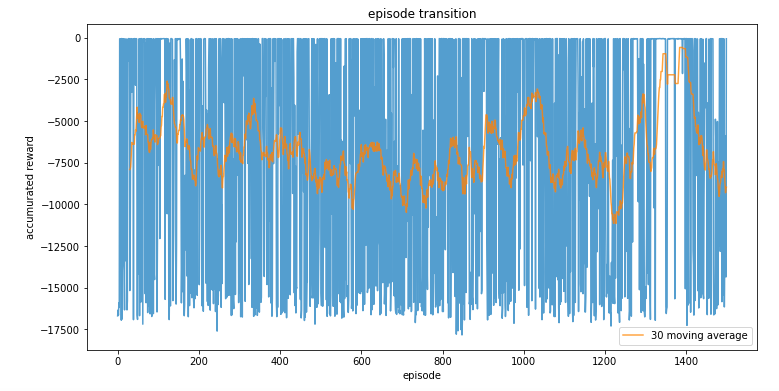
\includegraphics[width=12cm]{reward.png}
 	\caption{episode毎の蓄積reward} \label{reward}
\end{figure}
図\ref{reward}でも図\ref{pure_reward}と同じように全episodeを通してのrewardの変化をグラフにした. 30episode移動平均を見ても上昇していることは確認できないが, 図\ref{pure_reward}とは異なり, 0に近い値をとっている. これは振子を倒立させることに成功しているepisodeで確認されるrewardである. 図\ref{reward}と図\ref{pure_reward}のちがいは$U(s)$を如何に用いるかの違いなので, CBFによる強化学習は, 離散化による影響をどれだけ抑えられるのかに焦点を当てるべきかもしれない.

\subsection{課題}
離散化によって状態制約を満たさなくなってしまうトリガーがなにかわかっていないので, それについては今後の課題である.($\theta$ではなく$\dot{\theta}$による影響が強いのではないかと予想しています.)



\begin{thebibliography}{10}
\bibitem{event}
D. Baumann, J. J. Zhu, G. Martius, and S. Trimpe. “Deep Reinforcement Learning for Event-Triggered Control."  \textit{In Proc. of the 57th IEEE International Conference on Decision and Control}, 2018.
\bibitem{quad}
Li Wang, Evangelos A Theodorou, and Magnus Egerstedt. “Safe learning of quadrotor dynamics using barrier certificates," \textit{In 2018 IEEE International Conference on Robotics and Automation (ICRA)}, pages 2460-2465, 2018
\bibitem{safe}
R. Cheng, G. Orosz, R. M. Murray, and J. W. Burdick.  “End-to-end safe reinforcement learning through barrier functions for safety-critical continuous control tasks," \textit{Thirty-Third AAAI Conference on Artificial Intelligence}, 2019.

\end{thebibliography}

 
\end{document}